\chapter{Results}
\label{chap:results}

This section will provide the results from the data analysis of both the test of the agreement regarding the personality traits and characteristics, and the AttrakDiff evaluation to assess the user experience. The data was analysed using SPSS.

\section{Results from personality characteristics data analysis}

The characteristics were rated using a scale from 1-5 in which 5 meant a high perceived presence of the characteristic in the interaction with the chatbots, and 1 meant no perceived presence of the characteristics. The data-set was analysed through a two-way repeated measures ANOVA to investigate whether an interaction effect occurred within subjects, as all participants were subjected to all conditions.

The descriptive statistics of the characteristics data analysis can be found in table \ref{table:5}.

\begin{table}[h]
\centering
\begin{tabular}{cccccc}
\hline
\multicolumn{6}{c}{\textbf{Descriptive Statistics}} \\
\hline
& N & Minimum & Maximum & Mean & Std. Deviation \\
Extroversion_A & 16 & 2 & 5 & 4,3125 & 0,8116 \\
Extroversion_B & 16 & 1,67 & 3,33 & 2,2708 & 0,47483 \\
Agreeable_A & 16 & 4 & 5 & 4,625 & 0,30277 \\
Agreeable_B & 16 & 2,25 & 4,5 & 3,4219 & 0,57532 \\
Conscientious_A & 16 & 3,33 & 5 & 4,2917 & 0,5146 \\
Conscientious_B & 16 & 2,67 & 4,67 & 3,9167 & 0,60246 \\
Openness_A & 16 & 3 & 5 & 4,0781 & 0,59665 \\
Openness_B & 16 & 1,5 & 5 & 3,4531 & 0,92294 \\
\end{tabular}
 \caption{Descriptive statistics chatbot characteristics results}
 \label{table:5}
    \end{table}

A two-way repeated measures ANOVA was conducted that examined whether the starting condition had an interaction effect. The independent variable personality has two levels, and the dependent variable characteristics has four factors where each factor describes a factor from the five factor model (extroversion, agreeable, conscientiousness, openness). The two-way repeated ANOVA included a starting condition (startbot) to investigate whether the order of chatbots participants were subjected to had any effect on the results.

There was a significant main effect of the two levels of personality with respect to the characteristics F(1,14)=73,181, p<,001 and there was an INsignificant interaction effect between personality and the starting condition p=,926. There was also a significant main effect between the characteristics F(3,42)=12,960, p<,001, and an INsignificant effect between characteristics and starting condition p=,869. There was a significant interaction effect between personality and characteristics p<,001. There was an INsignificant interaction effect between the personality and characteristic and the starting order (personality*characteristics*startbot) p=,380. See figure \ref{fig:characstartAB}.

\begin{figure}[h]
    \centering
    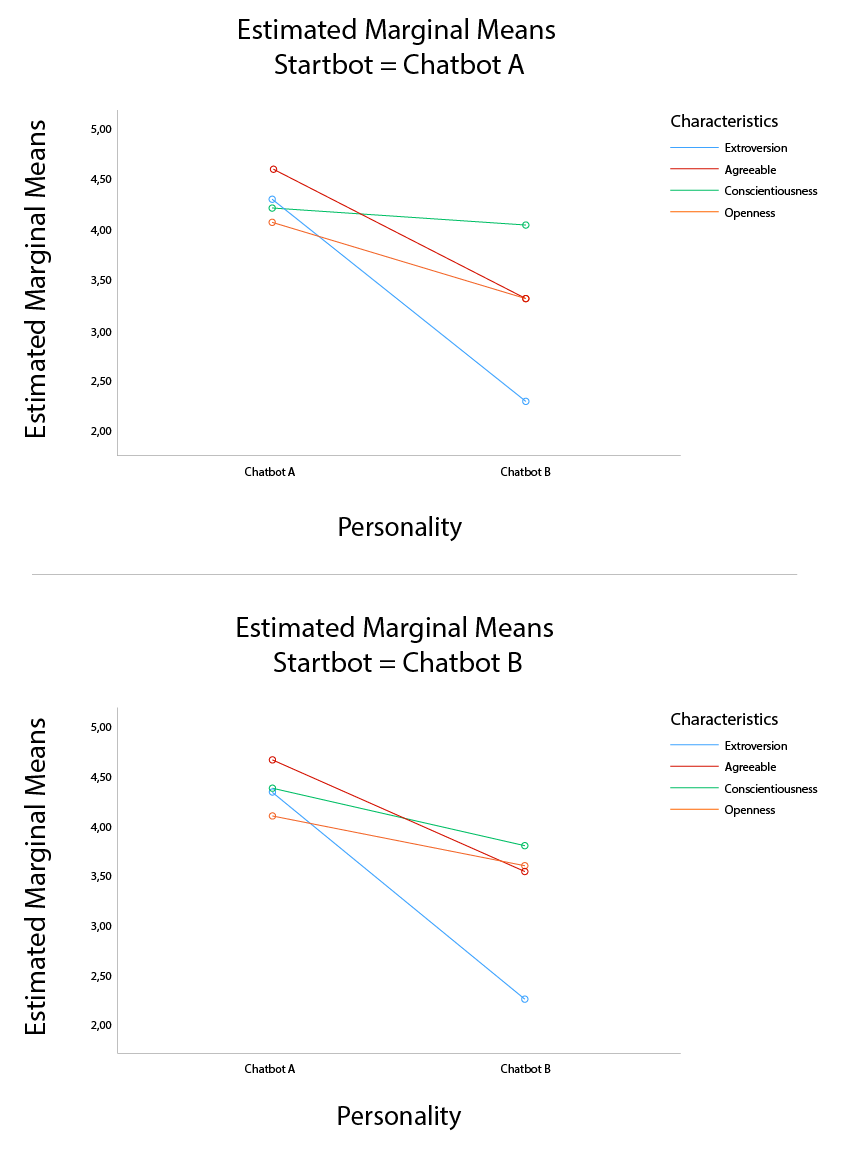
\includegraphics[scale=0.4]{figures/MMeanStartbotABCharacteristics.png}
    \caption{Estimated marginal means of characteristics starting condition Chatbot A and Chatbot B}
    \label{fig:characstartAB}
\end{figure}

The data was also tested for whether there was an interaction effect of gender. This tow-way repeated measures ANOVA revealed no significant interaction effect of gender (Personality*Characteristics*Gender) p=,331.

A paired-samples T-Test was conducted. The results found that there is a significant difference between the two levels of personality and the perceived characteristics. Agreeableness Chatbot B (M=3,4219, SD=,57532) and Chatbot A (M=4,6250, SD=,30277); t(15)=-8,760, p < ,001. Extroversion Chatbot B (M=2,2708, SD=,47483) and Chatbot A (M=4,3125, SD=,81166) t(15)=-8,976, p < ,001. Openness Chatbot B (M=3,4531, SD=,92294) and Chatbot A (M=4,0781 SD=,59665) t(15)=-3,727, p = ,002. Conscientiousness Chatbot B (M=3,9167, SD=,60246) and Chatbot A (M=4,2917, SD=,51460) t(15)=-2,522, p = ,023. These results suggests that participants perceived the two personalities as significantly different from one another. The Mean score difference between Chatbot B and A, suggests that participants perceived all characteristics in Chatbot A to a higher degree than in Chatbot B, where the extroversion factor had the largest difference in mean score.

\section{Results from AttrakDiff data analysis }
        
The data-set was analysed through a two-way ANOVA to understand whether an interaction effect occurred that could have an impact on how users rated either version. The analysis investigated the effect the independent variable personality had on the dependent variable user experience. Personality includes two levels, and user experience is made up of four factors (pragmatic, hedonic identity, hedonic simulation, attractiveness).

The descriptive statistics of the AttrakDiff data analysis can be found in table \ref{table:6}. Descriptive statistic for all word-pairs found in each factor can be found in Appendix \todo{appendix}.

\begin{table}[h]
\centering
\begin{tabular}{cccccc}
\hline
\multicolumn{6}{c}{\textbf{Descriptive Statistics}} \\
\hline
& N & Minimum & Maximum & Mean & Std. Deviation \\
PQ_A & 16 & 4,86 & 6,71 & 5,9286 & 0,56424 \\
PQ_B & 16 & 4 & 6,43 & 5,4732 & 0,5964 \\
HQ-I_A & 16 & 4 & 6,29 & 5,4821 & 0,53165 \\
HQ-I_B & 16 & 3,57 & 5,43 & 4,7679 & 0,56874 \\
HQ-S_A & 16 & 5,14 & 6,14 & 5,625 & 0,29909 \\
HQ-S_B & 16 & 2,57 & 6,57 & 4,7768 & 1,19405 \\
ATT_A & 16 & 5,14 & 7 & 6,3482 & 0,44864 \\
ATT_B & 16 & 3,9 & 6,3 & 5,339 & 0,7805 \\
\end{tabular}
\caption{Descriptive statistics AttrakDiff results}
 \label{table:6}
    \end{table}

A two-way repeated measures ANOVA was conducted to investigate the effect of the starting condition (startbot) had on the independent variable personality and the dependent variable user experience. Personality has two levels (personality, no personality) and user experience has four factors (pragmatic, hedonic stimulation, hedonic identity, attractiveness). The between-subjects factor (startbot), tested for any interaction effect dependent on which chatbot participants started with (chatbot A or Chatbot B).

There was a significant main effect of the two levels of personality with respect to the user experience F(1,14)=15,300, p=,002), and the between subject factor (startbot) had no significant interaction effect on personality p=,847. There was a significant main effect of the user experience F(3,42)=12,264, p<,001, and the start condition (startbot) had no significant interaction effect on user experience p=,865. There was no significant interaction effect between personality, user experience and start condition (personality*UXscore*startbot) p=,909. See figure \ref{fig:startA} and \ref{fig:startB}.

\begin{figure}[h]
    \centering
    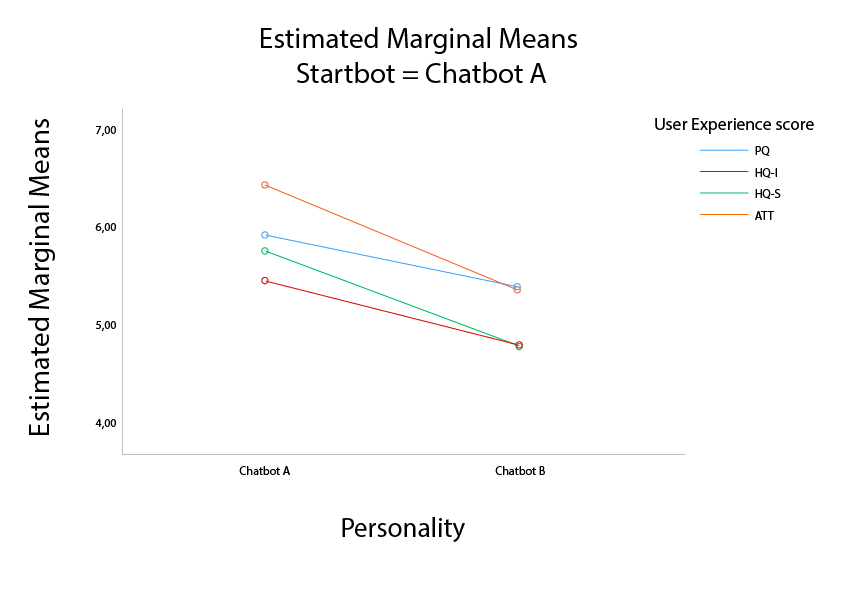
\includegraphics[scale=0.4]{figures/MMeanStartbotA.png}
    \caption{Estimated marginal means starting condition chatbot A}
    \label{fig:startA}
\end{figure}

\begin{figure}
    \centering
    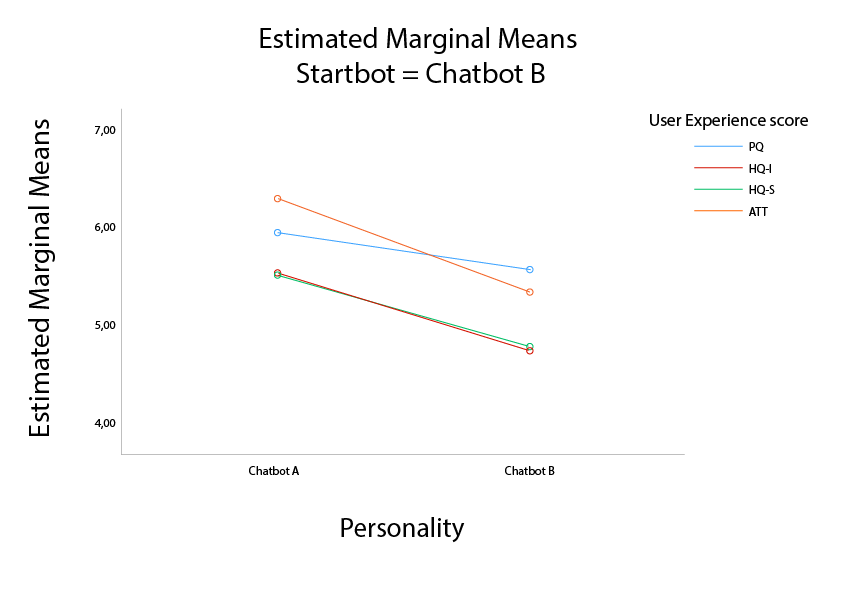
\includegraphics[scale=0.4]{figures/MMeanStartbotB.png}
    \caption{Estimated marginal means starting condition chatbot B}
    \label{fig:startB}
\end{figure}

Another two-way repeated measures ANOVA was conducted to investigate whether gender had any significant interaction effect on the variables. The analysis found that there was no significant interaction effect between personality, user experience and gender (personality*UXscore*gender) p=,436.

The paired samples t-test found that there is a significant difference in the scores between Chatbot B and Chatbot A, where all four factors of the user experience showed a significant improved effect between Chatbot B and A. Pragmatic Quality Chatbot B (M=5,4732, SD=,59649) and Chatbot A (M=5,9286, SD=56424); t(15)=-2,152, p = ,048. Hedonic-I Quality Chatbot B (M=4,7679, SD=,56874) and Chatbot A (M=5,4821, SD=,53165) t(15)=-3,239, p = ,006. Hedonic-S Quality Chatbot B (M=4,7768, SD=1,19405) and Chatbot A (M=5,6250 SD=,29909) t(15)=-2,934, p = ,010. Attractiveness Chatbot B (M=5,339, SD=,7805) and Chatbot A (M=6,3482, SD=,44864) t(15)=-4,069, p = ,001. These results suggests that personality has an improved effect on the user experience of chatbots, as all four factors of user experience was scored higher for chatbot A than chatbot B.

\begin{figure}[h]
    \centering
    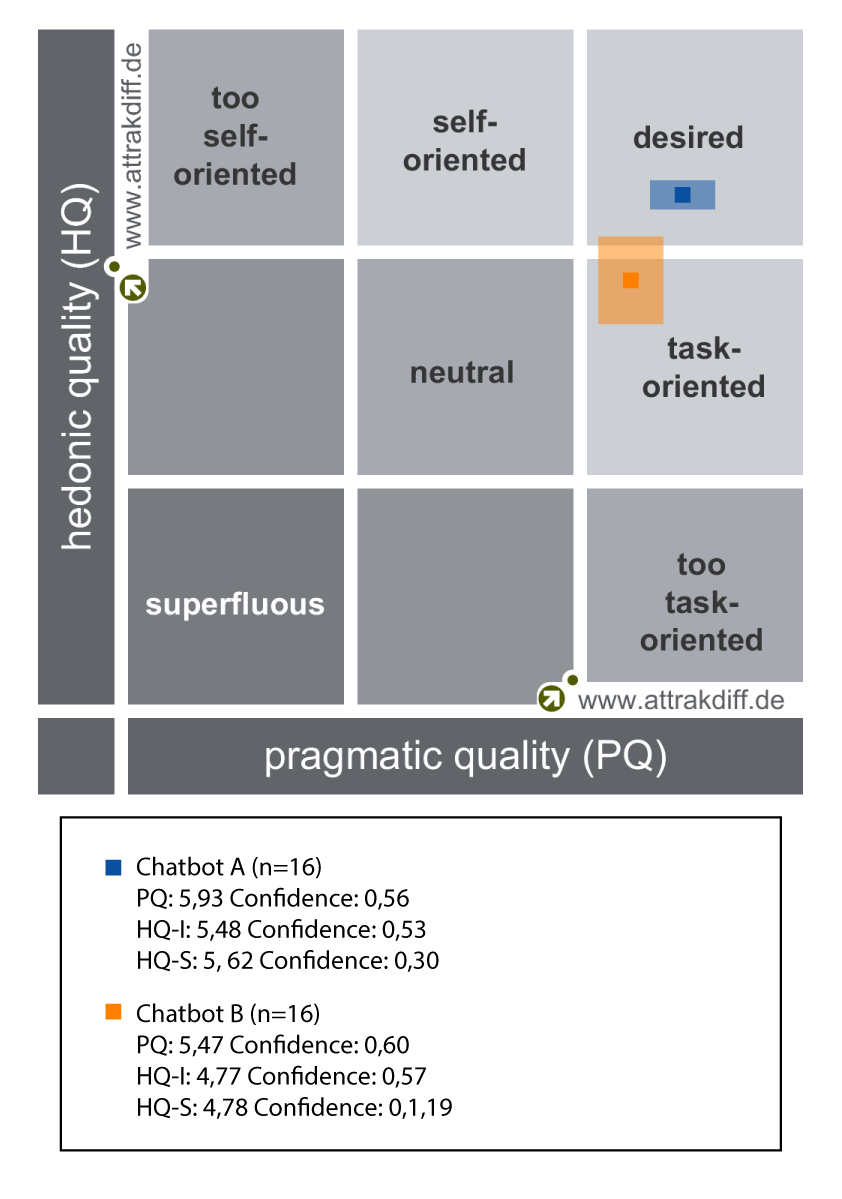
\includegraphics[scale=0.4]{figures/Portfolio-of-results-attrakdiff.png}
    \caption{Results Attrakdiff}
    \label{fig:portres}
\end{figure}
        
As shown in Figure \ref{fig:portres}, Chatbot A performed better in both hedonic and pragmatic quality than Chatbot B. The rectangles shows the confidence observed for Chatbot A and B, where Chatbot A has a smaller confidence rectangle implying that the participants were largely at one. Chatbot B however has a much larger confidence rectangle, which suggests that participant responses differed more greatly. Figure \ref{fig:diagval} shoes the means score of each user experience factor and how the two personalities scored compared to each other. The diagram shows that the difference is greater when it comes to hedonic quality-simulation and attractiveness, while the differences are less when it comes to pragmatic quality in particular. As the two personalities only shared traits found in the conscientiousness personality factor (reliable, consistent, perceptive) this result is to be expected as those traits are often found to be pragmatic qualities. Figure \ref{fig:wordpairs} shows the average score for each of the word-pairs for both chatbot versions. This line graph shows clearly where the differences are largest, such as human-technical, and that the for the majority of word-pairs Chatbot A scores higher. The exceptions includes mainly word-pairs in the pragmatic quality: cumbersome-straightforward, unpredictable-predictable, unprofessional-professional. This suggests that a technical, impersonal or machine-like personality are seen as more professional and straightforward than a more human-like personality.

\begin{figure}[h]
    \centering
    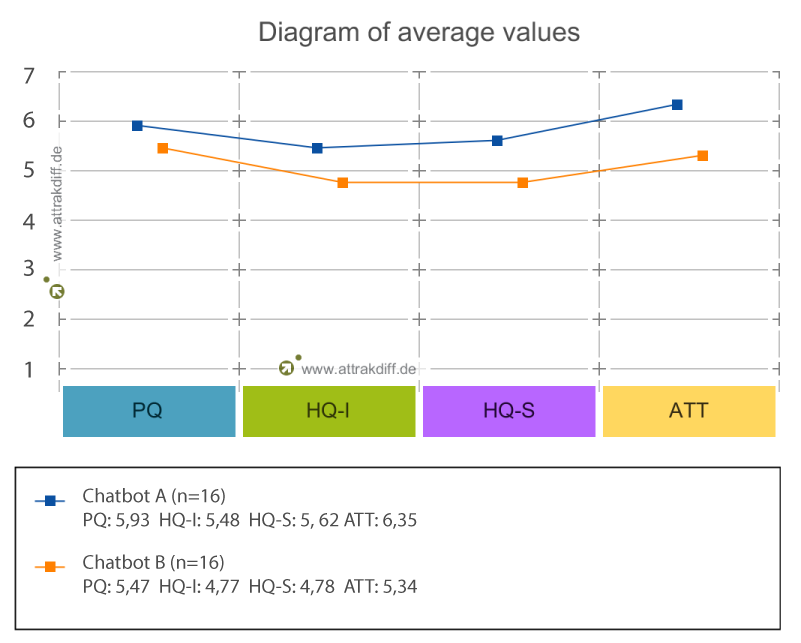
\includegraphics[scale=0.5]{figures/Diagram-of-average-values.png}
    \caption{Diagram of average values}
    \label{fig:diagval}
\end{figure}

\begin{figure}[h]
    \centering
    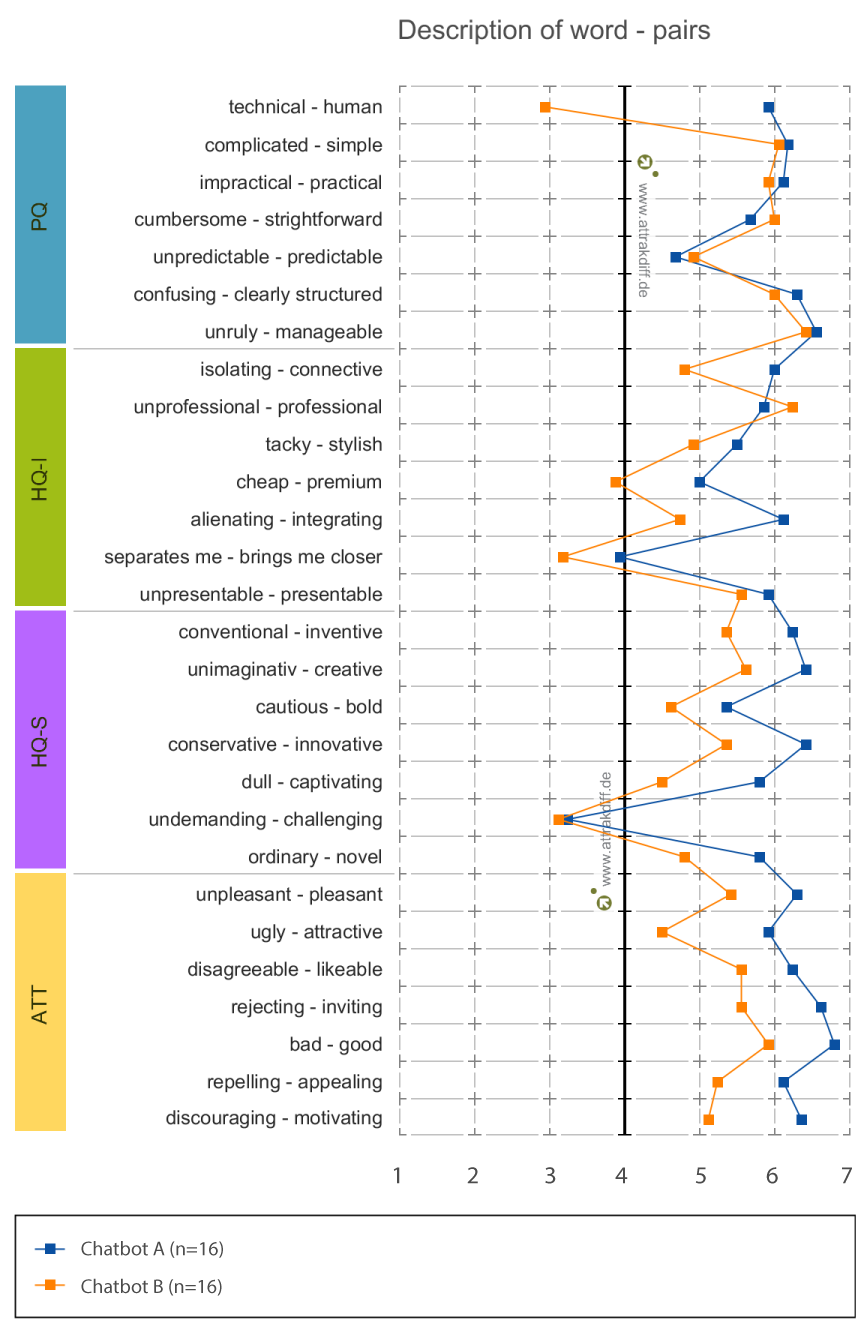
\includegraphics[scale=0.4]{figures/Description-of-word-pairs.png}
    \caption{Description of word-pairs}
    \label{fig:wordpairs}
\end{figure}